%%%%%%%%%%%%%%%%%%%%%%%%%%%%%%%%%%%%%%%%%%%%%%%%%%%%%%%%%%%%%%%%%%%%
%           Auteur :  P.TRAN BA, E.BOUTTIER, J.SHI, E.ABIA         %
%         Création :  18/01/2012 17:05                             %
%%%%%%%%%%%%%%%%%%%%%%%%%%%%%%%%%%%%%%%%%%%%%%%%%%%%%%%%%%%%%%%%%%%%

\documentclass[a4paper,11pt]{article}

%\usepackage[utf8]{inputenc}
%\usepackage[T1]{fontenc}
%\usepackage{xunicode}
\usepackage{fontspec}
\defaultfontfeatures{Mapping=tex-text,Scale=MatchLowercase}
\usepackage{a4wide}
\usepackage{verbatim}
\usepackage{polyglossia}
\setdefaultlanguage{french}
%~ \usepackage{listings}
%\usepackage[french]{babel}
%~ \usepackage{url}
%~ \usepackage{times}
\usepackage{minted}
\usepackage{amssymb}
\usepackage{graphicx}
% graphviz.tex
% originally written by Derek Rayside, November 2003
% following an idea that Daniel Jackson implemented in his Tagger program
%
% parameters to \digraph:
% 1 - parameters for \includegraphics (optional; default value is "scale=1")
% 2 - name of the digraph
% 3 - body of the digraph

\newcommand{\digraph}[3][scale=1]{
    \newwrite\dotfile
    \immediate\openout\dotfile=#2.dot
    \immediate\write\dotfile{digraph #2 {\string#3}}
    \immediate\closeout\dotfile
    \IfFileExists{#2.ps}
        % the postscript exists: include it
        { \includegraphics[#1]{#2} }
        % the postscript doesn't exist: tell the user how to create it
        { \fbox{ \begin{tabular}{l}
            The file \texttt{#2.ps} hasn't been created from
            \texttt{#2.dot} yet. \\
            Run `\texttt{dot -Tps -o #2.ps #2.dot}' to create it. \\
            Here is a \textsf{bash} loop to process all \textsf{dot} files
            in the current directory: \\
            \texttt{
            for f in *.dot do ; 
            dot -Tps -o \$\{f\%dot\}ps \$f ; 
            done
            }
            \end{tabular}}
        }
}



\usepackage{geometry}
\geometry{hmargin=2.5cm,vmargin=1.5cm}

\title{Projet C\\Simulation d'un commutateur de niveau 3\\Rapport}
\author{Philippe \textsc{Tran Ba}, Élie \textsc{Bouttier},
Jiajun \textsc{Shi}, Émilie \textsc{Abia}\\Groupe 15}
\date\today

\begin{document}

\maketitle

\begin{abstract}

Ce rapport porte sur un projet de programmation d'un commutateur de
niveau 3 en langage C. Il y est abordé le fonctionnement global du
programme, suivi des choix techniques effectués afin de palier aux
problèmes rencontrés. Il termine par une conclusion sur l'état du projet
et des améliorations qui pourraient y être apportées.

\end{abstract}

\tableofcontents

\newpage

\section{Introduction}
\subsection{Préface}

Dans le cadre de notre préparation au diplôme d'ingénieur en
Télécommunications et Réseaux, nous avons été amenés à effectuer notre
projet C de première année sous l'encadrement de Jérôme Ermont. Le but de
ce projet était surtout de nous faire manipuler le langage C et la
gestion de la mémoire mais il nous a également permis de modéliser une
solution réseau simple.

La commutation de paquets, technique utilisée dans le transfert de
données dans les réseaux informatiques, permet de rediriger les paquets
sur un lien physique particulier suivant des critères précis, avec
éventuellement une modification de ceux-ci. Au vue de notre formation,
le choix de la réalisation d'un simulateur de commutateur se trouve être
pertinent et intéressant.

Ce rapport est composé de deux parties. La première partie présente
l'application dans sa globalité, son fonctionnement. La seconde partie
est consacrée au détail de l'implémentation. Enfin nous conclurons sur
les apports personnels obtenus à la fin de ce projet.

\subsection{Rappel du sujet}

Nous avons effectué notre projet langage C de première année sous
l'encadrement de Jérôme Ermont. Il était question principalement de
simuler le fonctionnement d'un commutateur de niveau 3. 

Ainsi il s'agissait dans ce projet de simuler le fonctionnement d'un élément
réseau dont le rôle serait de recevoir des trames, de les assembler pour
reformer des paquets et d'effectuer par la suite la commutation de ces
paquets. Les paquets routés sont à nouveau fragmentés et les trames
obtenues sont stockées dans des queues selon leur priorité.

La première étape a été l'étude préalable de l'élément réseau impliqué,
il s'agissait d'assimiler les fonctionnalités attendues de celui-ci et
de, relativement à notre compréhension du sujet, réfléchir à un
algorithme.

Dans un second temps, après nous être mis d'accord sur le modèle retenu
nous nous sommes départagé le travail afin de gagner du temps.  

Nous avons ensuite regroupé nos travaux et avons modifié la structure
générale du programme afin de l'optimiser au maximum. 

Enfin, il faut remarquer que notre application peut encore évoluer : il
serait par exemple souhaitable que le commutateur soit capable de mieux
traiter les erreur (reprise sur erreur, renvoie...).

\section{Implémentation}
\subsection{Architecture globale de l'application}

Notre application ayant attrait au réseau, il est naturel de la
décomposer en modules indépendants, à l'image des couches du modèle OSI. De
plus, une telle décomposition rend notre solution évolutive. Il sera
aisé de remplacer un module ou d'en ajouter. Sa décomposition en module
assure aussi sa stabilité.

Le simulateur est lancé par la méthode \texttt{simulate} du module
\texttt{simulator}. Les paramètres de lancement sont obtenue par le
module \texttt{main}, en charge d'analyser les arguments de la ligne de
commande. La simulation est commandée par le fichier d'entrée, comportant
des instructions \texttt{IN} et des instruction \texttt{out}, dictant
l'entrée ou la sortie d'un paquet.

Lors de la lecture d'une instruction \texttt{IN}, le module
\texttt{trame} sera appelé afin de lire une trame depuis le fichier
d'entrée. Celle-ci est alors rangée dans une structure de données
nommé \texttt{ListPacketFrag}, en attendant d'obtenir toute les trames
d'un même paquet. C'est donc une liste chaîné, contenant dans chaque
cellule un \texttt{PacketFrag} – paquet fragmenté – contenant un tableau
de trame, rempli au fur et à mesure de leur arrivée. Lorsque toutes les
trames d'un même paquet sont reçues, le paquet fragmenté est retiré de la
liste \texttt{ListPacketFrag}, afin d'être envoyé au module
\texttt{packet}, en charge de l'assemblage. Le schéma ci-après résume
le stockage des données dans les différentes structures.

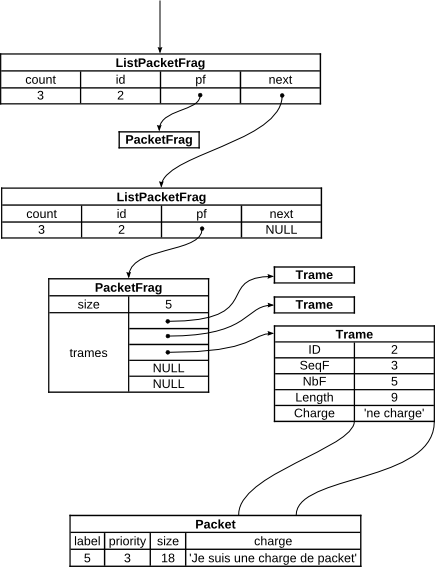
\includegraphics{s1.png}

Un paquet étant reconstitué, celui-ci est envoyé au module
\texttt{commut}, en charge de sa commutation. Celui-ci modifie son label
en concordance avec la table de commutation, et indique au simulateur le
lien de sortie. Celui-ci va alors demander au module \texttt{packet} de
le fragmenter, avant de l'envoyer dans la \texttt{queue} dédiée au lien
de sortie précédemment établi.

Lors d'une instruction \texttt{OUT}, le module \texttt{queue} est appelé
afin d'envoyer une trame sur le lien de sortie concerné et donc de
l'écrire dans un fichier de sortie. La trame sortie est sélectionnée
selon sa priorité de manière circulaire sauf la priorité absolue, qui
elle, est envoyée immédiatement après un \texttt{OUT}.

Le diagramme UML page suivante résume les différents modules utilisés
dans l'application ainsi que les relations qui les lient.

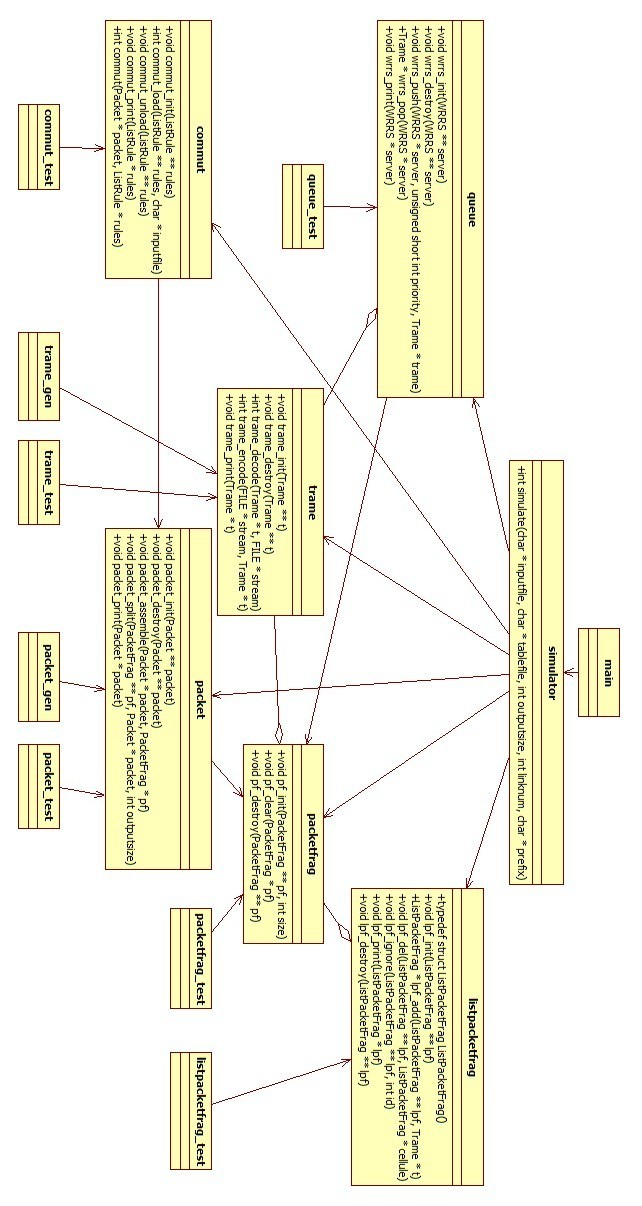
\includegraphics[height=27cm]{UML.jpg}

\subsection{Détail des modules}

\subsubsection{trame}
Le module \texttt{trame} propose une fonction de décodage dont le
prototype est le suivant :
\begin{minted}{c}
int trame_decode(Trame * t, FILE * stream);
\end{minted}
Son objectif est le décodage d'une trame depuis le fichier
\texttt{stream} afin de remplir la structure suivante :
\begin{minted}[linenos]{c}
typedef struct {
    unsigned short int id; /* numéro du paquet */
    unsigned short int seqf; /* numéro de séquence */
    unsigned short int nbf; /* nombre de séquence */
    unsigned int length; /* longeur de charge */
    unsigned char * charge; /* contenue */
} Trame;
\end{minted}
Cette fonction a été implémenté sous la forme d'une machine à états afin
de suivre l'avancement dans la lecture. L'état $9$ désigne la lecture du
fanion de fin de trame, tandis qu'un état négatif désigne la détection
d'une erreur.
\begin{minted}[linenos]{c}
while (state < 9 && state > -1) {
    pending = fgetc(stream); /* Lecture d'un caractère */
    if (pending == EOF) { /* On contrôle qu'il n'y ai pas eu d'erreur */
        fprintf(stderr, "trame_decode: error in fgetc\n");
        state = -1; 
    } else {
        switch (state) {
            // Action suivant l'état
        }
    }
}
\end{minted}
Par exemple, un des états est associé à la lecture des bits de poids fort
de l'ID de la trame. L'octet lu est alors décalé de 8 bits. L'état suivant
est associé à la lecture des bits de poids faible de l'ID. Pour obtenir
l'ID final, on utilise l'opération ou entre l'octet lu et les bits de poids
fort précédement décalé.

Tout au long du décodage, la CRC est calculé en effectuant un \textit{ou exclusif}
avec l'octet qui vient d'être lu. Si la CRC lue dans la trame n'est pas
identique, la trame est ignoré.
\begin{minted}{c}
crc ^= pending;
\end{minted}

Inversement, ce module propose une fonction d'encodage, servant cette
fois-ci à écrire les données contenues dans la structure \texttt{Trame}
dans un fichier. Voici son prototype :
\begin{minted}{c}
int trame_encode(FILE * stream, Trame * t);
\end{minted}


\subsubsection{packetfrag}
\texttt{packetfrag} correspond à un module gérant les fragments de paquets,
ou les trames d'un même paquet. Un paquet fragmenté contient, comme ci-dessous, 
une trame ainsi que la taille du paquet auquel elle appartient :
\begin{minted}{c}
struct PacketFrag {
    // Nombre de fragment (taille du tableau)
    int size;
    // Tableau contenant les trames
       Trame ** trames;
};
typedef struct PacketFrag PacketFrag;
\end{minted}


\subsubsection{listpacketfrag}
\texttt{listepacketfrag} est un module qui définit la structure des
maillons de la liste chainée qui contient les fragments de paquet.
\begin{minted}[linenos,tabsize=4]{c}
 struct ListPacketFrag {
    // Nombre de trame stocké dans le packet fragmenté
    int count;
    // ID du packet associé
    int id;
    // Packet fragmenté de la cellule
    PacketFrag * pf;
    // Cellule suivante
    struct ListPacketFrag * next;
};
typedef struct ListPacketFrag ListPacketFrag;
\end{minted}
\texttt{listepacketfrag} contient l'ID du paquet associé afin de savoir
si une trame appartient au paquet concerné ou non. Elle contient aussi
un compteur qui permet de savoir lorsque toute les trames d'un paquet
sont arrivées dès que celui-ci atteint le nombre de séquence.

Cette liste chaînée est utilisée afin de stocker les paquets fragmentés
avant leur assemblage. Il propose donc des fonctions d'ajout de trame,
et de retrait de paquet fragmenté (lorsque le paquet est assemblé) dont
les prototypes sont les suivants :
\begin{minted}[linenos,tabsize=4]{c}
ListPacketFrag * lpf_add(ListPacketFrag ** lpf, Trame * t);
void lpf_del(ListPacketFrag ** lpf, ListPacketFrag * cellule);
\end{minted}


\subsubsection{packet}
\texttt{Packet} est un module contenant la structure qui représentera à
nos yeux un paquet défini comme ci dessous:
\begin{minted}[linenos,tabsize=4]{c}
 struct Packet {
  unsigned int label;
  unsigned char priority;
  unsigned int size;
  unsigned char * charge;
};
typedef struct Packet Packet;
\end{minted}
Ce modules est aussi chargé de l'assemblage et de la re-fragmentation du
paquet en de multiple trames via les deux fonctions qui suivent :
\begin{minted}[linenos,tabsize=4]{c}
/* Assembler un packet */
void packet_assemble(Packet * packet, PacketFrag * pf);
/* Fragmenter un packet */
void packet_split(PacketFrag ** pf, Packet * packet, int outputsize);
\end{minted}




\subsubsection{commut}
\texttt{commut} est le module qui gère la table de commutation de notre
appareil. Cette dernière est définie ainsi :
\begin{minted}{c}
 /* Liste chaîné des règles de commutation */
struct ListRule {
    unsigned int inlabel;
    unsigned int outlabel;
    int outlink;
    struct ListRule * next;
};
typedef struct ListRule ListRule;
\end{minted}
Pour charger la table de commutation, nous utiliserons :
\begin{minted}{c}
 /* Charger les règles de routage depuis un fichier */
int commut_load(ListRule ** rules, char * inputfile);
\end{minted}
Puis, la fonction :
\begin{minted}{c}
 /* Commuter un packet.
 * Change le label et renvoit le lien de sortie.
 * Renvoit -1 si le packet n'est concerné par aucune règle. */
int commut(Packet * packet, ListRule * rules);
\end{minted}
Qui elle, renvoie le lien de sortie et modifie le label du paquet.




\subsubsection{queue}
\texttt{Queue} est un module gérant les files d'attentes avec gestion
des priorité. Une queue est une liste chaînée de trames :
\begin{minted}{c}
 struct Queue {
    struct Queue * previous;
    Trame * element;
};
typedef struct Queue Queue;
\end{minted}
Chaque queue sera attribuée à une priorité. Dans notre cas, 256 priorités
sont gérées, et chaque queue associée est stockée dans une cellule d'un
tableau de 256 queues, l'indice représentant la priorité.
Ce tableau est contenu dans une structure WRRS ci dessous :
\begin{minted}{c}
 /* Weighted Rount Robin Server */
struct WRRS {
    Queue * queue[NBPRIORITY]; // Tableau des queues de trame (une par
    priorité)
    int priority; // Priorité en cours
    int credit; // Nombre de crédit pour la priorité en cours
};
typedef struct WRRS WRRS;
\end{minted}
L'ajout de trame se fait par le biais de la fonction de la fonction
\texttt{wrrs\_trame}.
\begin{minted}{c}
/* Ajouter une trame dans le serveur */
void wrrs_push(WRRS * server, unsigned short int priority, Trame * trame);
\end{minted}
Les variables \texttt{priorité} et \texttt{credit} dans le WRRS
contiennent les informations nécessaires à l'application de l'algorithme
de décision lors de la sortie d'une trame. Celui-ci est déclenché par
l'appel de la fonction \texttt{wrrs\_pop} dont voici le prototype :
\begin{minted}{c}
/* Obtenir la prochaine trame devant sortir du serveur.
 * Retourne NULL si le server est vide. */
Trame * wrrs_pop(WRRS * server);
\end{minted}

\subsubsection{main}
La méthode \texttt{main} se contente de récupérer les arguments. Après
avoir vérifié leurs validité, ils les fait passer au module
\texttt{simulator} pour lancer la simulation. Il vérifie également la
validité des paramètres, comme une  aussi la validité des données.

\subsubsection{simulator}
\texttt{simulator} est le coordinateur des autres modules
précédemment énoncés. Il est appelé par la méthode \texttt{main} et
s'occupe du fichier d'entré. Il s'occupe également de
charger la table de commutation par le biais du module \texttt{commut}.
Tout comme \texttt{trame\_decode}, il implémente une machine à état pour
la lecture du fichier d'entrée. Deux sous-programme, \texttt{in} et
\texttt{out} s'occupent des actions a effectuer à la lecture de « IN »
ou de « OUT ».

La fonction \texttt{in} va tous d'abord décoder une trame avant de
l'envoyer dans la structure de stockage temporaire en attendant
l'assemblage. S'il s'agit de la dernière trame manquante d'un paquet,
les trames associées sont retirées de la liste pour être assemblées. Le
paquet est ensuite commuté, fragmenté, et envoyé dans la file d'attente
associé à son lien de sortie.

La fonction \texttt{out} appelle la fonction \texttt{wrrs\_push} sur la
file d'attente associée au lien de sortie demandé. La trame ainsi
récupérée est écrite dans le bon fichier par le biais de 
\texttt{trame\_encode}. Afin de n'ouvrir que les fichiers nécessaire, et
de ne pas devoir les ré-ouvrir à chaque écriture d'une trame sur un même
lien de sortie, un tableau static est utilisé. Celui-ci comporte une
cellule par lien de sortie, contenant un pointeur de type \texttt{FILE *}
sur le fichier en question. Au premier appel de la fonction, les pointeurs
sont \texttt{NULL}, et ils sont initialiser au fur et à mesure des
différents appels de la fonction lorsqu'un lien est solicité.
\begin{minted}{c}
static FILE ** streams = NULL; // Fichiers de sortie
if (streams == NULL) { calloc(linknum, sizeof(*streams)); }
if (streams[link] == NULL) { // Le fichier n'a pas encore été ouvert
    sprintf(filename, "%s-%d", prefix, link);
    streams[link] = fopen(filename, "a");
}
trame_encode(streams[link], t);
\end{minted}



\section{Réalisation du projet}

\subsection{Difficultés et solutions}

Au départ, le stockage dans l'ordre des trames semblait bien difficile. Un tableau dynamique n'était pas simple à manipuler mais nous ne pouvions pas mettre de tableau fixe. Nous avons réalisé que lorsque l'on recevait une trame, on savait directement le nombre de trame que l'on recevrait grâce à l'attribut \textit{nbf}. Ainsi il semblait bien plus simple d'allouer directement un tableau de la bonne taille et ranger les trames dans le bon ordre.

\subsubsection{Solutions envisageable}

Plusieurs solutions ont été proposées lors de l'étude du cahier des charges. Dans la mesure où il nous était demandé de ne pas nous focaliser sur les performances mais plutôt sur le choix des structures de données et l'efficacité des algorithmes.

Au départ nous comptions gérer les trames dans une partie décodage, gérer les paquets dans une partie assemblage et gérer la queue dans une partie éponyme.
 
Dans la partie décodage nous avions défini une structure de données Trame, une liste chaînée de trames utilisée pour stocker les trames d'un même paquet qui n'est pas encore complet et une liste de « Paquets Fragmentés » ListePacketFrag utilisée pour stocker les différentes listes de trame.


Nous avions alors envisagé que les opérations disponibles sur une trame pourraient être :
Créer une trame à partir d'un numéro de paquet, d'un numéro de séquence, d'un nombre de séquence, de la longueur d'une charge, d'une somme de contrôle et d'un contenu.
\begin{enumerate}
 \item Initialiser une trame
 \item Transformer une séquence de bits en trame
 \item Transformer une trame en une séquence de bits
 \item Vérifier si un ID existe
 \item Ajouter une trame dans la ListeTrame
 \item Ajouter une ListeTrame dans la ListePacketFrag
 \item Vérifier si la ListeTrame est complète
 \item Vérifier si la Trame est correcte en utilisant CRC
 \item Calculer CRC
\end{enumerate}

C'est dans la partie assemblage que nous avions défini la structure Packet et les opérations disponibles sur un paquet, la plus importante étant bien sûr le décodage de la trame dans le but de l'intégrer à un paquet.

Puis dans la partie queue nous avions envisagé que la queue serait un tableau de taille 256, soit le nombre maximal de priorité. 

\subsubsection{Difficultés rencontrées et solution retenue}

Comme le calcul de la CRC ne tient pas compte de la CRC originale suivant la charge, donc les difficultés concernant cette procédure sont :
\begin{enumerate}
 \item Comment faire un calcul de CRC en excluant la CRC originale.
 \item Comment faire un calcul de CRC dans le cas où la CRC originale est égale à un fanion ou un banaliseur.
\end{enumerate}


\vspace{0.5cm}

Pour le problème 1 :

Selon la formule :

A = A xor B xor B

On sait qu'il suffit de faire une fois \textit{ou exclusif} avec le CRC original et le CRC calculé incluant CRC original, on peut obtenir un CRC  en excluant le CRC original.

Pour le problème 2 :

Si la CRC reçu est un fanion ou un banaliseur, c'est qu'on a
 calculé la crc aussi sur le banaliseur qui précédait la crc reçu.

Donc on doit faire encore une fois \textit{ou exclusif} avec le banaliseur.


Comme il n'y pas de mécanisme de gestion d'exception comme JAVA pour langage C, on utilise un type de retour INT pour indiquer l'état d'exécution afin de contrôler les erreurs.
On a décider un code de retour tel que si 0, ça veut dire qu'il n'y pas d'erreur, -1 sinon.

\vspace{0.5cm}

Ainsi, partant de la volonté de développer une application efficace, nous avons effectué grand nombre de modifications. La plus significative concernant la structure de donnée qui stocke les trames lorsqu'un paquet n'est pas encore complet. En effet, nous sommes passés d'une liste de liste à une liste de tableau.

\section{Conclusion}

Pour mener à bien ce projet de première année, nous avons dû approfondir nos connaissances en terme d'analyse de trame. Nous nous sommes aussi documenté sur le fonctionnement des protocoles TCP/IP afin de s'en inspirer.

De plus, ce projet nous a permis de nous familiariser avec la démarche de création d'un programme complexe ainsi  que des notions vues en réseaux. En effet, nous avons développé cette application par un travail de groupe, ce qui nous attend en tant que futurs ingénieurs. Plusieurs personnes travaillant sur un même programme ont besoin d'énormément de coordination et de synchronisation. Cela s'est révélé bien plus difficile que prévu, outre la standardisation de nos variables et la répartition des modules.

La partie que nous avons développée correspond aux objectifs de départ. Les résultats de simulation sont tout à fait satisfaisants tant au niveau routage qu'au niveau gestion de la mémoire. Savoir faire des simulations et le faire tout le long du projet est un outil précieux afin de corriger les erreurs le plus vite possible avant que celles-ci ne se répercutent sur la suite.

Le projet que nous avons réalisé cette année peut encore évoluer.
En effet, la gestion des trames perdues ou erronées est très limitée.
Il pourrait être envisagé d'étendre le protocole afin de permettre de la
reprise sur erreur. Par exemple, nous pourrions une ajouter fonctionnalité qui détruirait la trame si aucune autre trame du même paquet 
n'arrive dans un délai imparti. Ceci permet de recevoir un paquet de
même ID qui arriverait plus tard. Une autre voie d'évolution est la
gestion de plusieurs liens entrants, avec éventuellement une table de
commutation qui en tiendrait compte. Il serait également intéressant de
passer à une version asynchrone permettant la réception et l'émission de
trame simultanément.

\end{document}
